%% !TEX program = lualatex
%% !TEX TS-program = lualatex
% !TEX encoding = UTF-8 Unicode
% !TEX spellcheck = en_GB
\documentclass{beamer}

\usepackage{multirow}

% \graphicspath{{./graphics/}}

% ====================
% Packages
% ====================

\usepackage[T1]{fontenc}
\usepackage{lmodern}
% \usepackage[size=a4,scale=1.1]{beamerposter}
\usepackage[size=a1,scale=1.0]{beamerposter}
% \usepackage[size=custom,height=100,width=70.71,scale=1.2]{beamerposter}
% \usepackage[size=a4,scale=1.0,orientation=landscape]{beamerposter}

\usetheme{gemini}
\usecolortheme{poster}
\usefonttheme{default}

\usepackage{graphicx}
\usepackage{booktabs}
\usepackage{tikz}
\usepackage{pgfplots}
\pgfplotsset{compat=1.17}
\usepackage{multicol}
% \usepackage{enumerate}
% \usepackage{enumitem}
\usepackage{caption}
\captionsetup{font=normalsize}
% ====================
% Lengths
% ====================

% If you have N columns, choose \sepwidth and \colwidth such that
% (N+1)*\sepwidth + N*\colwidth = \paperwidth
% \colwidth = 1pt * \ratio{\paperwidth - {\ncols+1}\sepwidth}{\ncols}
\newcommand{\ncols}{3}
\newlength{\sepwidth}
\newlength{\colwidth}
\newlength{\midspace}
\setlength{\sepwidth}{0.020\paperwidth}
% \setlength{\colwidth}{0.32\paperwidth}
\setlength{\colwidth}{
{\dimexpr \paperwidth / \ncols \relax} -
{\dimexpr \sepwidth + \sepwidth / \ncols \relax}
}
\setlength{\midspace}{20ex}

\newcommand{\separatorcolumn}{\begin{column}{\sepwidth}\end{column}}

% ====================
% Title
% ====================

\title{Software Interface Design for a Full-Duplex Embedded System}

\author{\textbf{Student:} Taharka Okai}

\institute[shortinst]{University of Bristol, Dept. of Engineering}

\newcommand{\beamerblocknoheader}{
  \setbeamertemplate{block begin}{
    {\parskip0pt\par}
    \usebeamerfont{block body}
    \vskip-0.5ex
    \begin{beamercolorbox}[colsep*=0ex]{block body}
    \justifying
    \setlength{\parskip}{1ex}
    \vskip-2ex
  }

  \setbeamertemplate{block alerted begin}{
    % \begin{beamercolorbox}[colsep*=0ex,dp=2ex,center]{block alerted title}
    %   \vskip0pt
    %   \usebeamerfont{block title}\insertblocktitle
    %   \vskip-1.25ex
    %   \begin{beamercolorbox}[colsep=0.025ex]{block alerted separator}\end{beamercolorbox}
    % \end{beamercolorbox}
    {\parskip0pt\par}
    \usebeamerfont{block body}
    \vskip-0.5ex
    \begin{beamercolorbox}[colsep*=0ex]{block alerted body}
    \justifying
    \begin{adjustwidth}{1ex}{1ex}
    \setlength{\parskip}{1ex}
    \vskip-2ex
  }
}

\newcommand{\beamerblockheader}{
\setbeamertemplate{block begin}{
\begin{beamercolorbox}[colsep*=0ex,dp=2ex,center]{block title}
  \vskip0pt
  \usebeamerfont{block title}\insertblocktitle
  \vskip-1.25ex
  \begin{beamercolorbox}[colsep=0.025ex]{block separator}\end{beamercolorbox}
\end{beamercolorbox}
{\parskip0pt\par}
\usebeamerfont{block body}
\vskip-0.5ex
\begin{beamercolorbox}[colsep*=0ex]{block body}
\justifying
\setlength{\parskip}{1ex}
\vskip-2ex
}

\setbeamertemplate{block alerted begin}{
\begin{beamercolorbox}[colsep*=0ex,dp=2ex,center]{block alerted title}
  \vskip0pt
  \usebeamerfont{block title}\insertblocktitle
  \vskip-1.25ex
  \begin{beamercolorbox}[colsep=0.025ex]{block alerted separator}\end{beamercolorbox}
\end{beamercolorbox}
{\parskip0pt\par}
\usebeamerfont{block body}
\vskip-0.5ex
\begin{beamercolorbox}[colsep*=0ex]{block alerted body}
\justifying
\begin{adjustwidth}{1ex}{1ex}
\setlength{\parskip}{1ex}
\vskip-2ex
}
}


% ====================
% Footer (optional)
% ====================

\footercontent{
  % \href{https://www.example.com}{https://www.example.com} \hfill
  % ABC Conference 2025, New York --- XYZ-1234 \hfill
  % \href{mailto:a.kalay@example.com}{a.k@example.com}
}


\abovefooter{
  % \hfill\includegraphics[height=9ex]{uoblogo.png}
}
% (can be left out to remove footer)

% ====================
% Logo (optional)
% ====================

% use this to include logos on the left and/or right side of the header:
% \logoright{\includegraphics[height=2cm]{uoblogo.png}}
% \logoleft{\includegraphics[height=5pt]{graphics/uoblogo.png}}

\hypersetup{
  pdfauthor={Taharka Okai},
  pdftitle={Designing a Sketch Based Interface for Electronic Circuit Simulation},
  pdfsubject={Poster},
  pdfkeywords={Electronic Circuit Simulation, Sketch Recognition, Computer Vision, Machine Learning},
  pdfstartview={FitH},
  pdfpagemode={UseOutlines},
  pdfpagelayout={SinglePage},
  pdfborder={0 0 0},
}

\renewcommand{\baselinestretch}{1.1}
\hyphenpenalty=10000

\date{\today}

\begin{document}

\begin{frame}[t]
  \begin{columns}[t]

    \separatorcolumn

    \begin{column}{\colwidth}
      \begin{block}{1. Project Background}
        Simulation is a well-known and useful computer-aided design (CAD) tool for
        analysing electronic circuits. However, ease of use and speed of prototyping
        are two major drawbacks of circuit simulation using traditional CAD tools.

        Additionally, there is an increasing trend in the use of machine learning
        tools to aid research and development \cite{review/Moreno-Garcia2019}. It
        is therefore desirable to develop a tool that uses machine learning to aid
        researchers and students in the design of electronic circuits.
      \end{block}

      \begin{block}{2. Existing Solutions}
        There are a number of existing solutions that are similar to the project
        outcome. These methods each have their own merits and drawbacks, as detailed
        below:

        \begin{itemize}
          \item \textbf{Programmatic}:
                \cite{alg/Shane2009}: using properties of the shapes of the components to identify
          \item \textbf{Support Vector Machines}:
                \cite{svm/Chen2019}: using a Support Vector Machine (SVM) to classify
          \item \textbf{Object Detection}: \cite{dl/Rachala2022,dl/Dey2021}: using deep learning with object detection
        \end{itemize}

        These approaches either require intimate knowledge of the geometry of the components
        and the image processing techniques required to extract the relevant information
        from the sketch, or do not provide a complete product that provides a simulation from
        the input image.
      \end{block}

      \begin{block}{3. Aims and Objectives}
        This project aims to produce a software tool that receives hand-drawn
        circuit diagrams as input and generates an LT-SPICE simulation file as output,
        which will be paired with a compatible backend to produce a circuit simulation.
        The user will be able to:

        \begin{itemize}
          \item Create a hand-drawn schematic using a sketching interface
          \item Pass the sketch to the application via camera or file upload
          \item Observe the resulting simulation on their device
        \end{itemize}
      \end{block}

      {
      %   \beamerblocknoheader
      % \vspace*{2ex}
      \begin{block}{4. Evaluation}
        The object detection phase of this project uses You Only Look Once (YOLOv8) \cite{dl/ultralytics},
        a state-of-the-art object detection algorithm, evaluated using the mean average
        precision (mAP) metric. The metric requires the ground truth bounding boxes to
        overlap with the predicted bounding boxes by a certain amount, known as the
        intersection over union (IoU) metric. The mAP metric is calculated as follows:

        $$
          \begin{aligned}
            \text{IoU} = \frac{A_{\text{intersection}}}{A_{\text{union}}} = \frac{A_{\text{intersection}}}{A_{\text{ground truth}} + A_{\text{prediction}} - A_{\text{intersection}}}
            \\[2ex]
            \text{mAP@0.5} = \frac{1}{N} \sum_{i=1}^{N} \text{AP}_i, \text{given IoU} > 0.5
          \end{aligned}
        $$

        This metric is a balanced measure of the model's ability to make correct predictions, (precision)
        but also how thoroughly it is able to detect all instances of the object in the image (recall).
        During training, this metric is one of the maximisation goals, which ensures that the
        model is able to make accurate, consistent predictions.
      \end{block}
      }


      % {\beamerblocknoheader
      % \vspace*{2ex}
      % \begin{block}{}
      %   \begin{figure}[t]
      %     \centering
      %     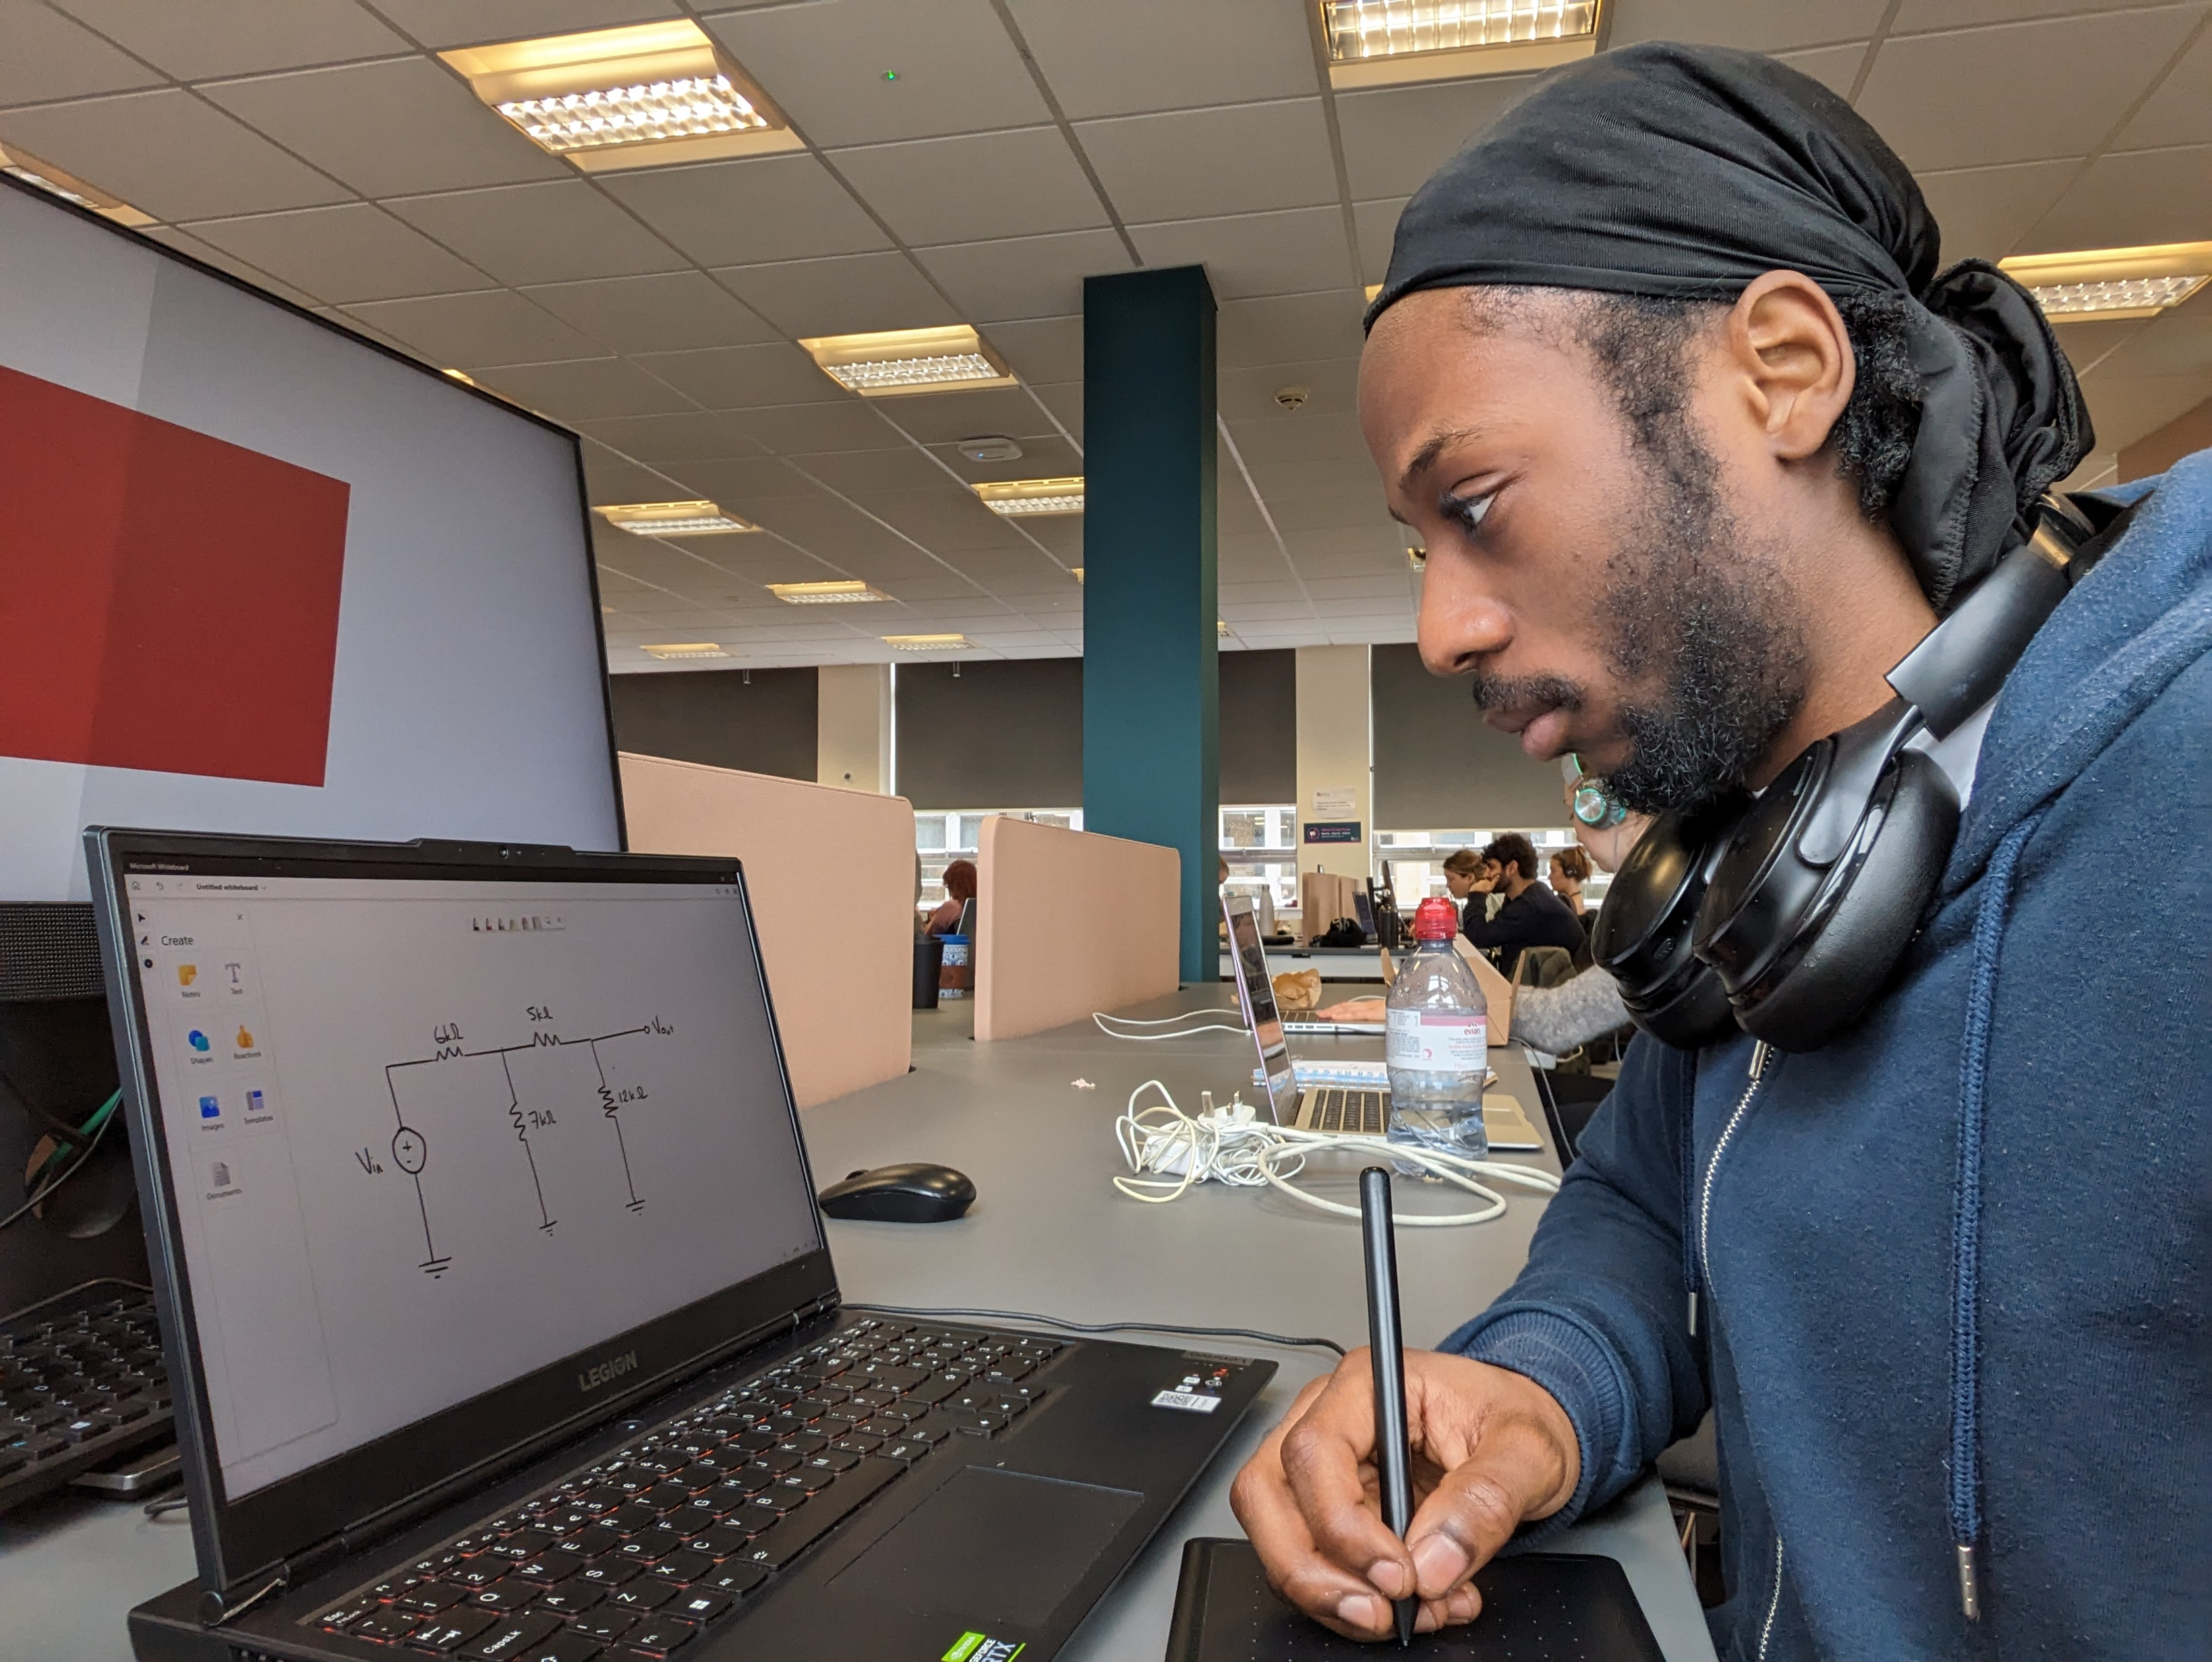
\includegraphics[keepaspectratio,width=\colwidth,height=35ex]{../common/graphics/demonstration-draw.jpg}
      %     % \resizebox{\colwidth}{!}{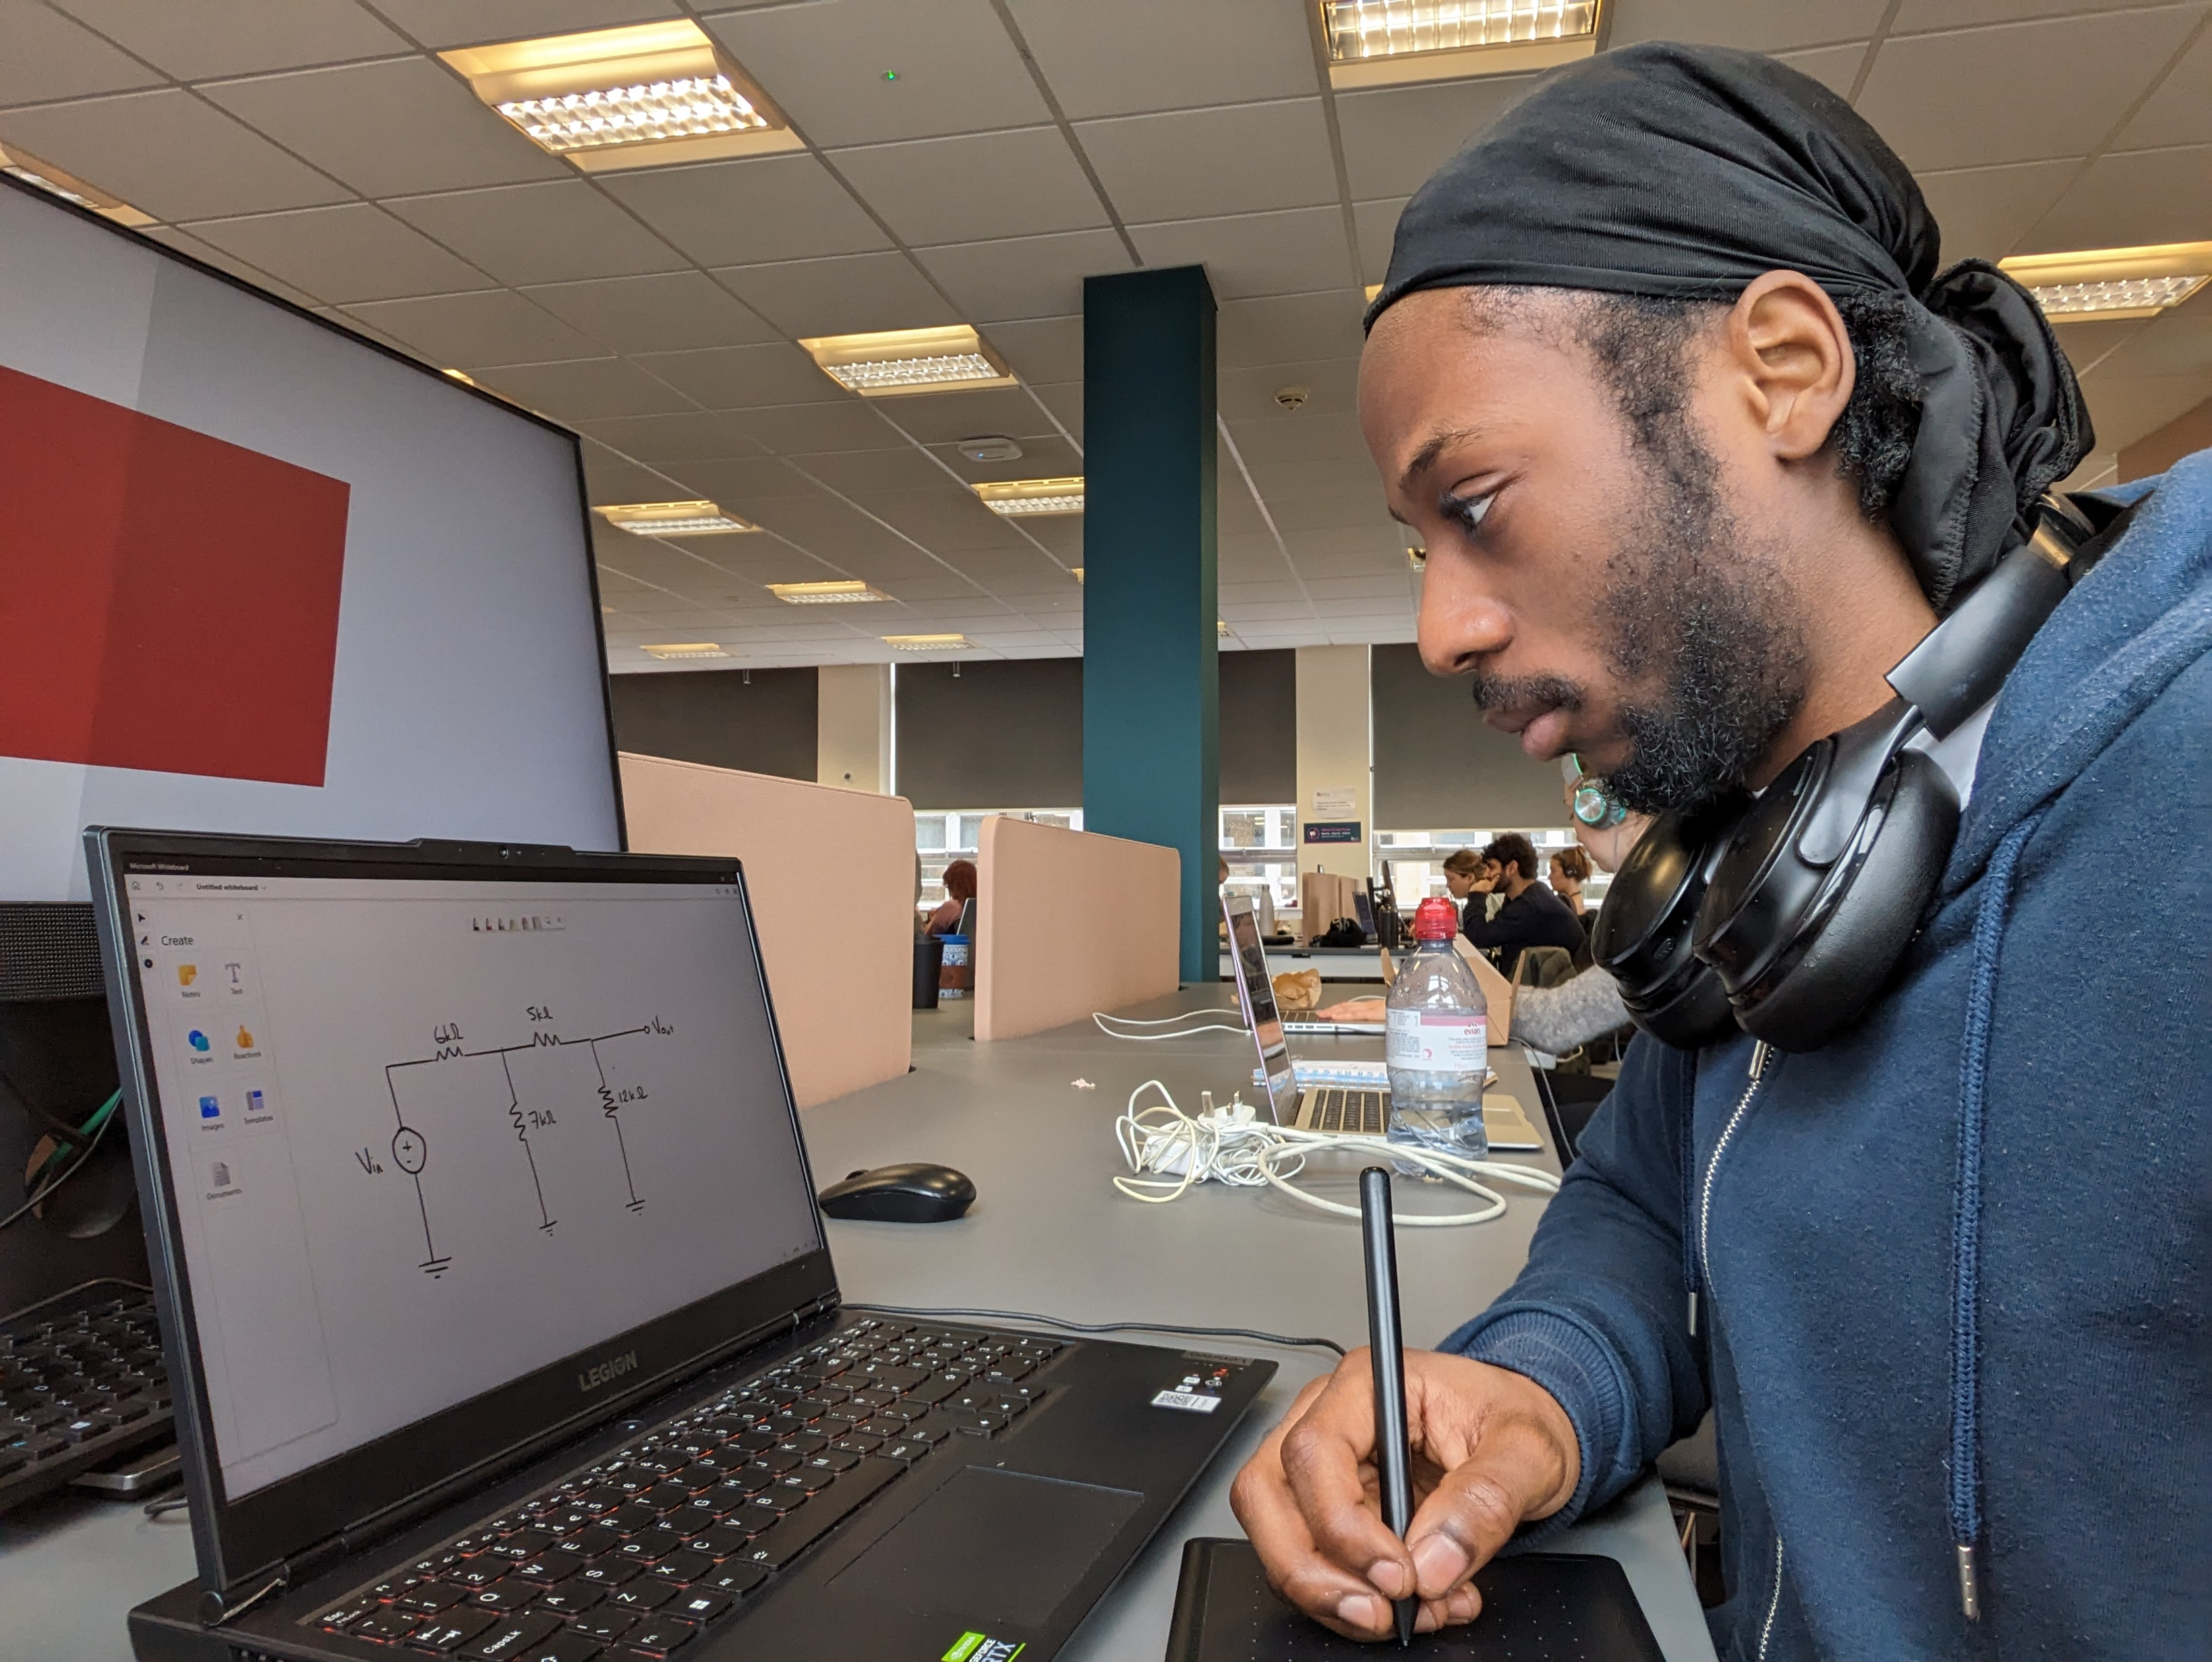
\includegraphics{../common/graphics/demonstration-draw.jpg}}
      %     \caption{Creating a digital image of the circuit diagram}
      %     \label{key1}
      %   \end{figure}
      % \end{block}
      % }

    \end{column}

    \separatorcolumn

    \begin{column}{\colwidth}
      % {\beamerblocknoheader
      %   \begin{block}{}
      %     \centering
      %     \begin{figure}[t]
      %       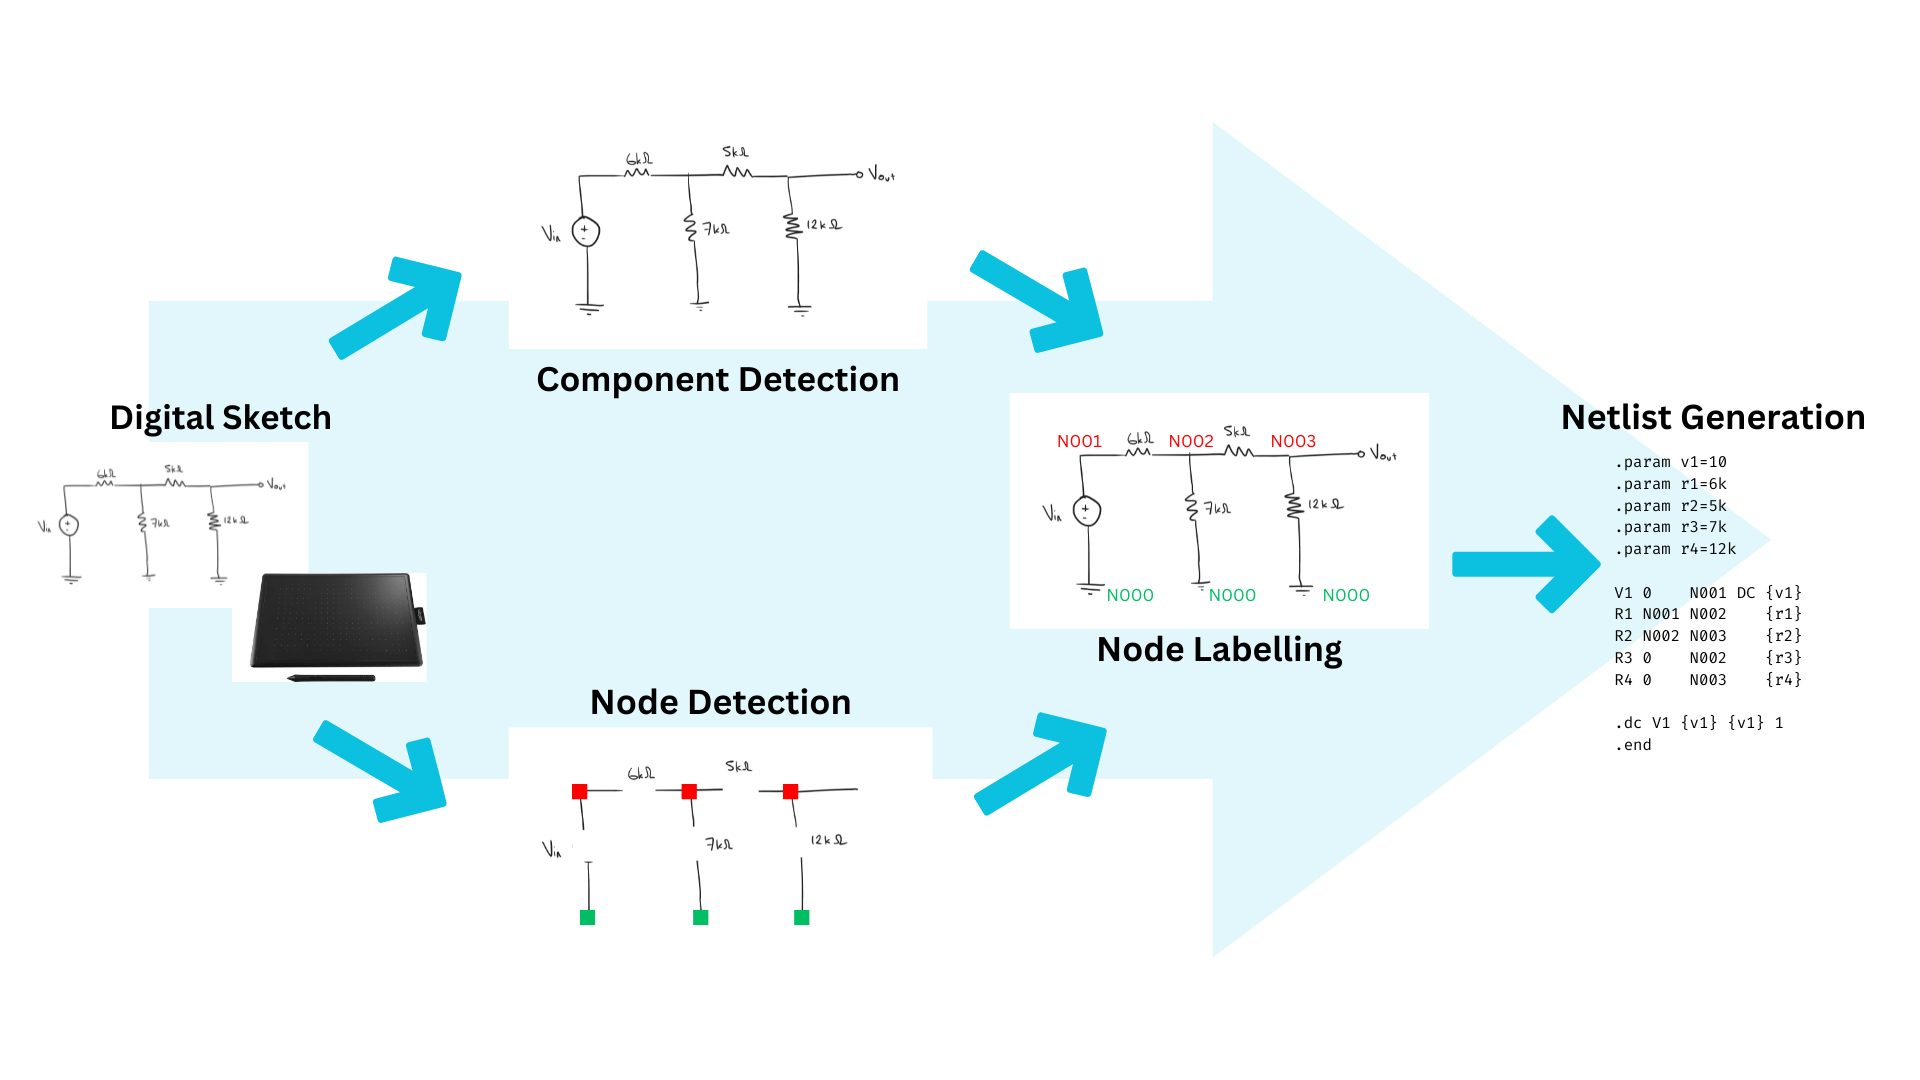
\includegraphics[height=35ex]{../common/graphics/create-representation}
      %       \caption{Creating a representation of the circuit diagram in software}
      %       \label{ke2}
      %     \end{figure}
      %   \end{block}
      % }



      {\beamerblocknoheader
        \begin{block}{}
          \begin{figure}[t]
            \centering
            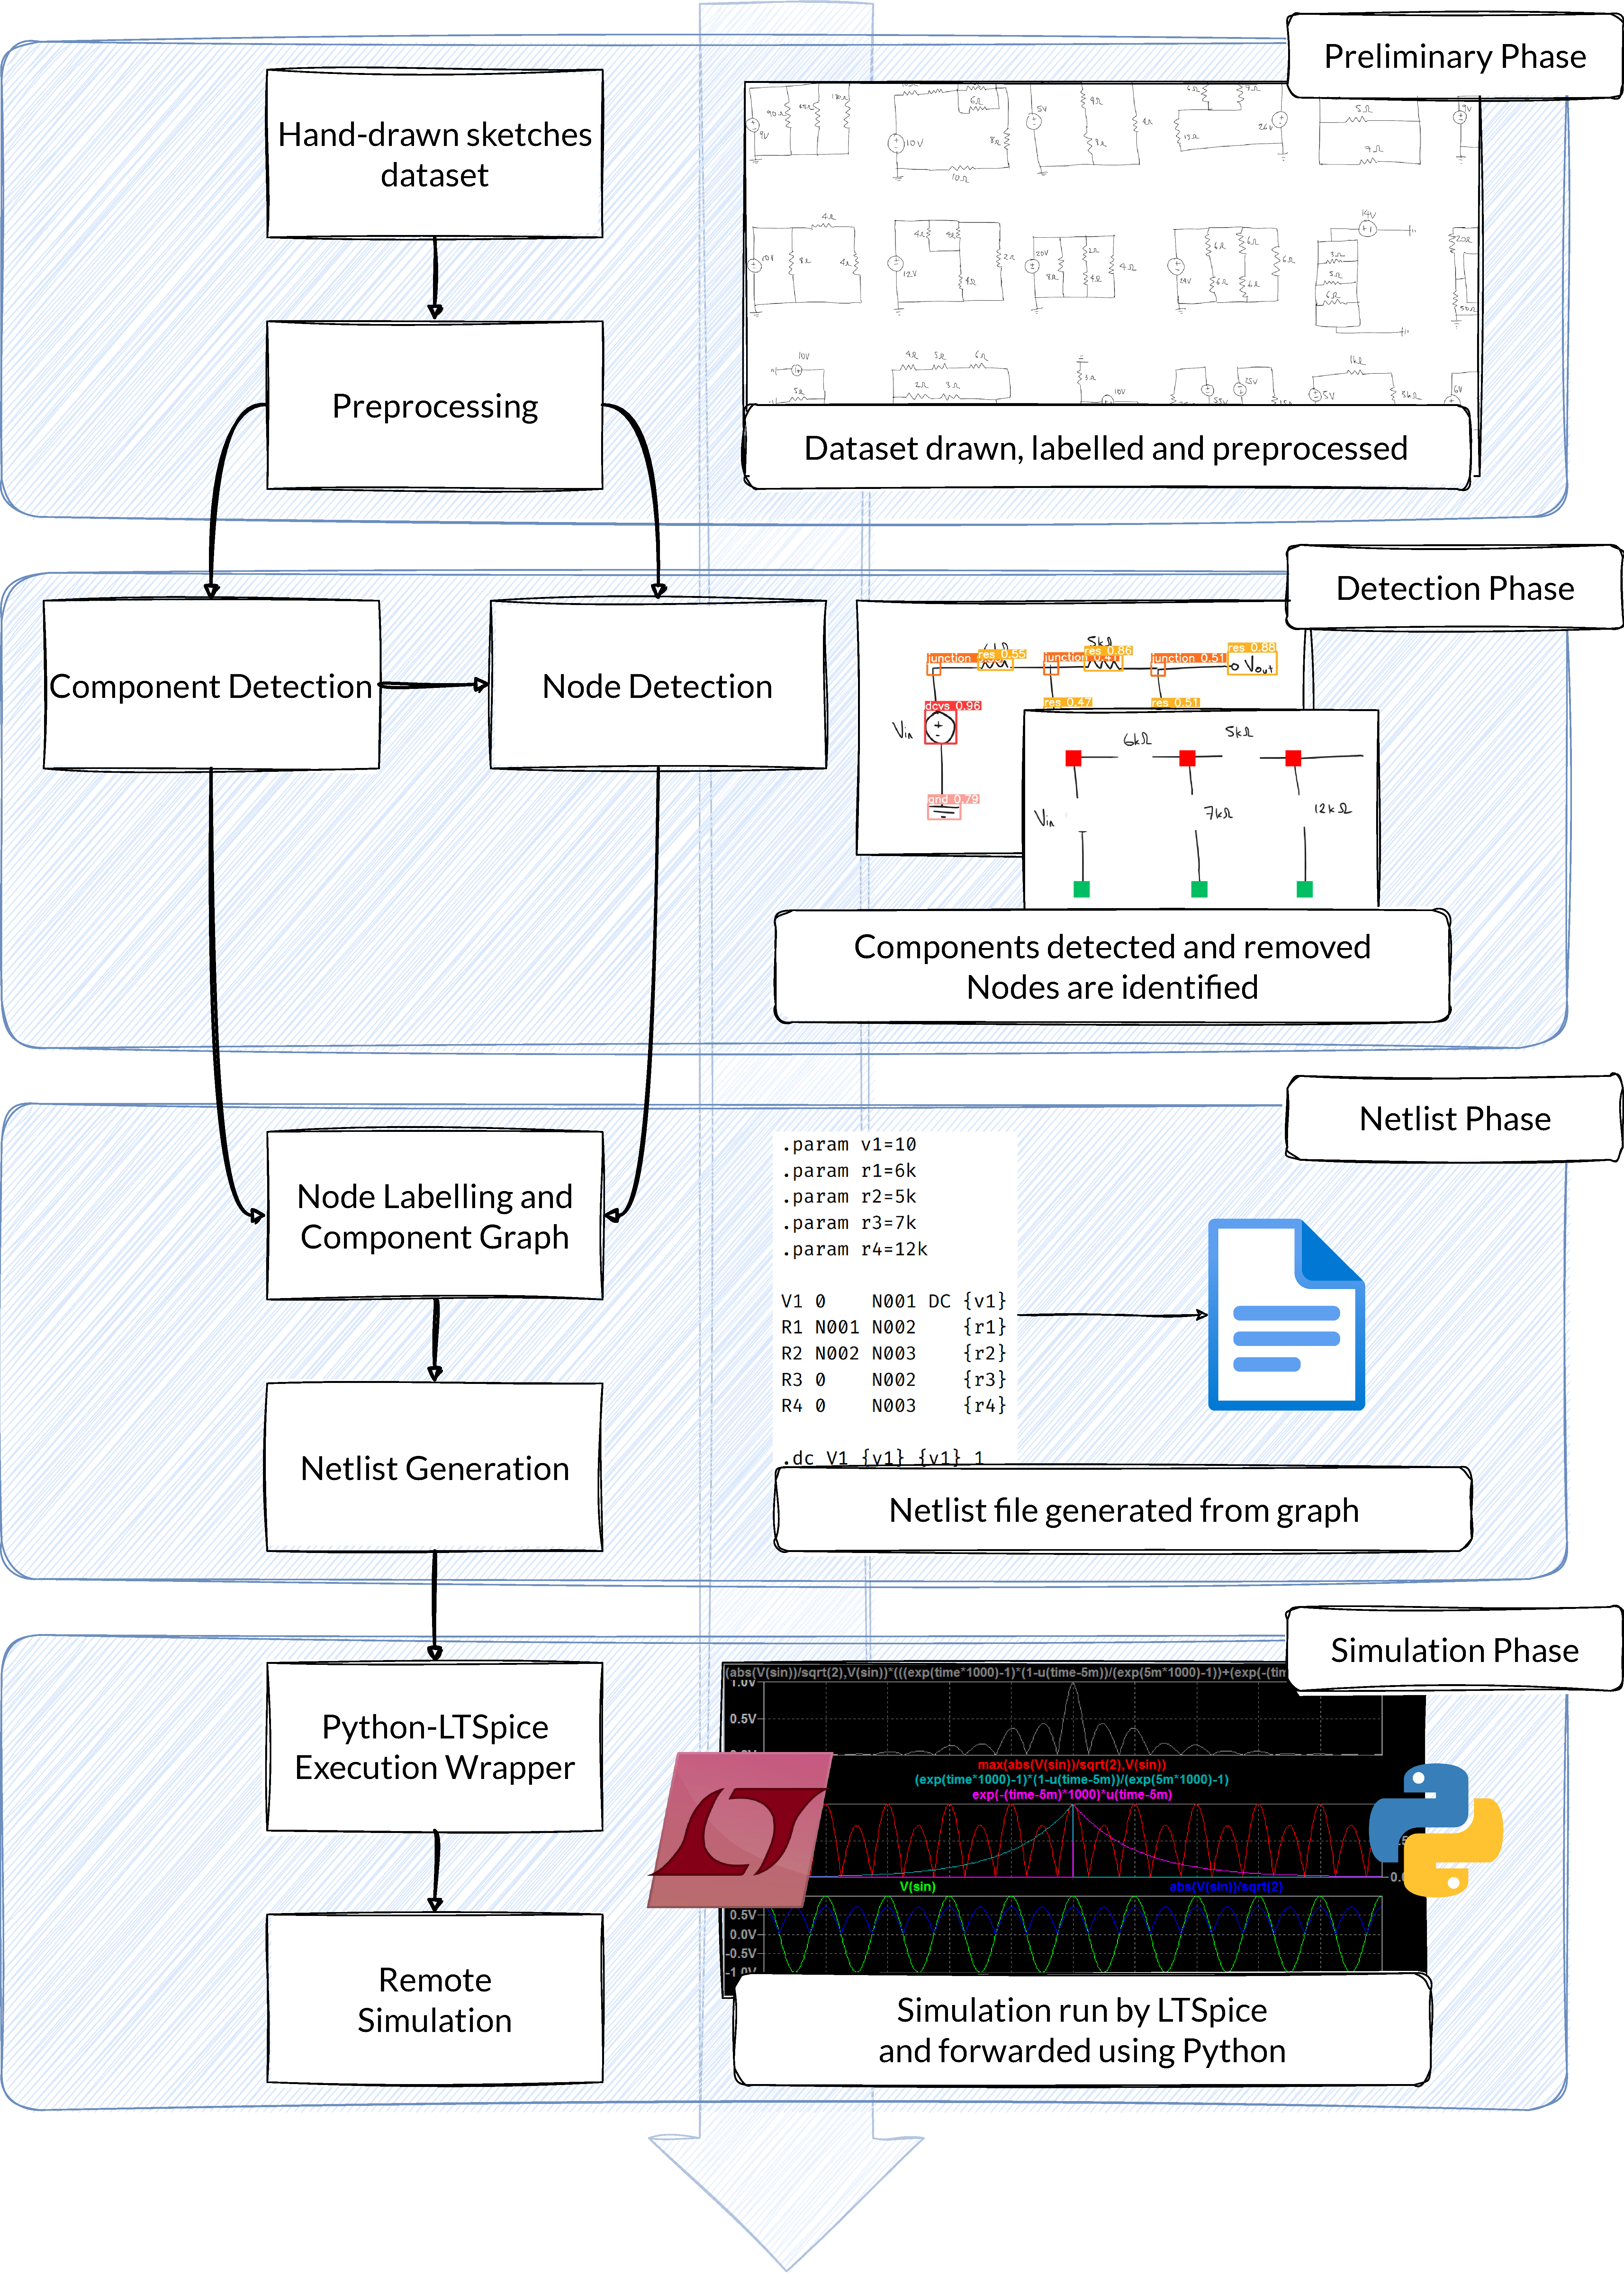
\includegraphics[keepaspectratio,width=\colwidth]{../common/graphics/methodology-1}
            \caption{Circuit sketch recognition method and simulation pipeline}
            \label{fig:methodology}
          \end{figure}
        \end{block}
      }

      {\beamerblocknoheader
        \begin{alertblock}{}
          \centering
          \begin{column}{\colwidth-\sepwidth}
            {\beamerblockheader
              \setbeamercolor{block body}{bg=,fg=white}
              \setbeamercolor{block title}{bg=,fg=white}
              \setbeamercolor{block separator}{bg=white}
              \setbeamertemplate{itemize item}{\raise0.5ex \hbox{{\color{white}\vrule width 0.5ex height 0.5ex}}}
              \setbeamertemplate{itemize subitem}{\raise0.3ex \hbox{{\color{white}\vrule width 0.5ex height 0.5ex}}}
              \RaggedRight

              \begin{block}{5. Method Brief}
                As outlined in Figure~\ref{fig:methodology}, the hand-drawn schematics are preprocessed
                and then passed to the deep learning object detection algorithm to detect the components
                of the circuit. The output of the detector is then passed to a post-processing stage to
                extract the netlist from the detected components. The netlist is then passed to Python
                and LT-SPICE to generate and run a simulation file.
              \end{block}
            }
          \end{column}
        \end{alertblock}
      }
    \end{column}

    \separatorcolumn

    \begin{column}{\colwidth}

      \setlength\tabcolsep{10pt}
      \renewcommand{\arraystretch}{1.5}

      {\beamerblocknoheader
        \begin{block}{}
          \begin{table}[t]
            \centering
            \begin{subtable}{0.90\textwidth}
              \centering\small
              \begin{tabular}{@{}lccc@{}}
                \toprule
                \textbf{Class}             & \textbf {Precision} & \textbf {Recall} & \textbf{mAP@0.5} \\
                \midrule
                \textbf{Resistor}          & 0.995               & 1.000            & 0.995            \\
                \textbf{DC Voltage Source} & 0.989               & 1.000            & 0.993            \\
                \textbf{Ground}            & 0.961               & 1.000            & 0.994            \\
                \textbf{Overall}           & 0.982               & 1.000            & 0.994            \\
              \end{tabular}
              \caption{Accuracy metrics for each class}
              \label{tab:accuracy-metrics}
            \end{subtable}

            \begin{subtable}{0.90\textwidth}
              \centering\small
              \begin{tabular}{@{}clcccc@{}}
                \toprule
                \multicolumn{2}{c}{\multirow{2}{*}{\textbf{Class}}}                & \multicolumn{4}{c}{\footnotesize Actual}                                                                                        \\
                                                                                   &                                          & \textbf{Resistor} & \textbf{DC Voltage Source} & \textbf{Ground} & \textbf{Not Data} \\
                \midrule
                \multirow{4}{*}{\rotatebox[origin=c]{90}{\footnotesize Predicted}} & \textbf{Resistor}                        & 1.00              & 0.00                       & 0.00            & 0.09              \\
                                                                                   & \textbf{DC Voltage Source}               & 0.00              & 1.00                       & 0.00            & 0.73              \\
                                                                                   & \textbf{Ground}                          & 0.00              & 0.00                       & 1.00            & 0.18              \\
                                                                                   & \textbf{Missed Data}                     & 0.00              & 0.00                       & 0.00            & 0.00              \\
              \end{tabular}
              \caption{Confusion matrix}
              \label{tab:confusion-matrix}
            \end{subtable}
            \caption{Evaluation metrics of the trained model}
            \label{tab:evaluation}
          \end{table}
        \end{block}
      }

      \vspace*{-3ex}

      \begin{block}{6. Findings, Ongoing and Future Work}
        A hand-drawn dataset of 100 images was created and used to train the model.
        Each image contained 3 component classes $\{res,dcvs,gnd\}$. Tables~\ref{tab:accuracy-metrics}
        and~\ref{tab:confusion-matrix} show the model achieves a precision and recall of over 98\% for $\{res,dcvs\}$,
        and 96\% for $\{gnd\}$. The confusion matrix reflects this, showing that the model
        accurately predicts all classes 100\% of the time.

        The trained detector can also function with reasonable accuracy directly on CAD images.
        This is demonstrated in a video linked as a \textbf{QR code at the end of this poster}.

        \begin{itemize}
          \item \textbf{Ongoing Work:}
                \begin{itemize}
                  \normalsize
                  \item[--] Interpret the circuit diagram and produce a simulation file.
                  \item[--] Run the simulation using a Python interface to LT-SPICE.
                  \item[--] Implement the user interface.
                \end{itemize}
          \item \textbf{Future Work:}
                \normalsize
                \begin{itemize}
                  \normalsize
                  \item[--] Increase the set of detectable components such as amplifiers and transistors.
                  \item[--] Detect text labels to avoid false positive detections.
                  \item[--] Integrate optical character recognition (OCR) to automate the netlist phase.
                \end{itemize}
        \end{itemize}
      \end{block}
      
      \vspace*{-2.5ex}

      {\beamerblocknoheader
      \begin{block}{}
        \footnotesize
        \bibliography{../common/sources}
        \bibliographystyle{IEEEtran}
      \end{block}
      }
      % \end{block}

    \end{column}

    \separatorcolumn

  \end{columns}

\end{frame}

\end{document}